%% ============================================================================
%% Supplementary Material: Paper 2 — Resistance-Informed MD Validation
%% Target: JCIM Supplementary Information
%% ============================================================================

\documentclass[11pt,a4paper]{article}
\usepackage[a4paper,margin=2.5cm]{geometry}
\usepackage[T1]{fontenc}
\usepackage[utf8]{inputenc}
\usepackage{lmodern}
\usepackage{amsmath, amsfonts, amssymb}
\usepackage{graphicx}
\usepackage{booktabs, tabularx, array, multirow}
\usepackage[table]{xcolor}
\usepackage[authoryear,round]{natbib}
\usepackage[hypertexnames=false,colorlinks=true]{hyperref}
\usepackage{cleveref}
\usepackage{xr}
\externaldocument[MAIN-]{Polypharmacology_MD_Validation_V2607}
\usepackage{siunitx}
\DeclareSIUnit\kcalmol{kcal\,mol^{-1}}
\DeclareSIUnit\angstrom{\text{\AA}}

\graphicspath{{../Graphics/}}

\title{Supplementary Information for \\ ``Resistance-Aware Polypharmacology of Antimalarial Leads \\
from African Natural Products: Docking, Network Scoring, and Targeted Molecular Dynamics''}
\author{Myke Vital Sao Temgoua\\
Jean-Pierre Tchapet Njafa\\
Serge Guy Nana Engo\\
Penabei Samafou\\
Wilfred Fon Mbacham}
\date{}

\begin{document}
\emergencystretch=2em
\maketitle

% ============================================================================
% Table S0: Docking Validation
% ============================================================================
%% ============================================================================
%% Table S0: Docking Protocol Validation — Enrichment Metrics
%% Target: JCIM Supplementary Information
%% Note: Data to be populated upon completion of enrichment studies.
%% Columns: Target, Method, ROC-AUC, EF1%, EF5%, BEDROC, Redocking RMSD (Å)
%% ============================================================================

\begin{table}[htbp]
\centering
\caption{Docking protocol validation: enrichment metrics and re-docking accuracy for the four wild-type targets. Active compounds were sourced from ChEMBL (IC\textsubscript{50} < 1~$\mu$M); decoys from DEKOIS 2.0 (1:4 active:decoy ratio). ROC-AUC, enrichment factors (EF\qty{1}{\percent}, EF\qty{5}{\percent}), and BEDROC ($\alpha = 80.5$) are reported for AutoDock Vina 1.2.7, Gnina 1.1 CNN-affinity, and their consensus (rank-normalised average). Re-docking RMSD is the heavy-atom RMSD between the top-scoring docked pose and the co-crystallised ligand.}
\label{tab:s0_docking_validation}
\begin{tabular}{l l S[table-format=1.3] S[table-format=1.2] S[table-format=1.2] S[table-format=1.3] S[table-format=1.2]}
\toprule
Target & Method & {ROC-AUC} & {EF\qty{1}{\percent}} & {EF\qty{5}{\percent}} & {BEDROC} & {RMSD (\si{\angstrom})} \\
\midrule
PfDHFR (7F3Y) & Vina & & & & & \\
& Gnina & & & & & \\
& Consensus & & & & & \\
\midrule
PfCRT (6UKJ) & Vina & & & & & \\
& Gnina & & & & & \\
& Consensus & & & & & \\
\midrule
PfATP4 (9N10) & Vina & & & & & \\
& Gnina & & & & & \\
& Consensus & & & & & \\
\midrule
PfClpP (4GM2) & Vina & & & & & \\
& Gnina & & & & & \\
& Consensus & & & & & \\
\bottomrule
\end{tabular}
\end{table}


% ============================================================================
% Figure S1: MPO Sensitivity Heatmap
% ============================================================================
\begin{figure}[htbp]
\centering
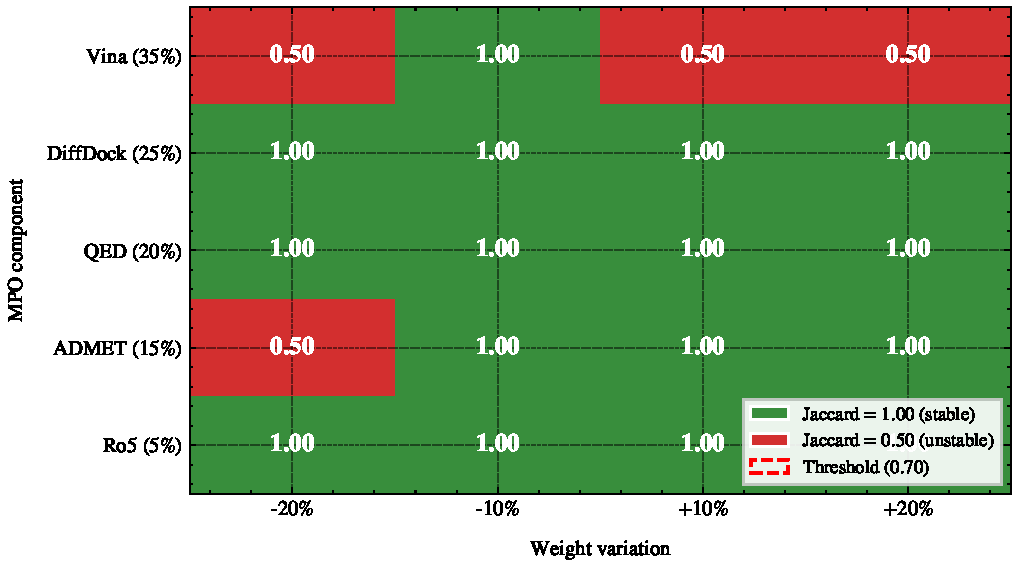
\includegraphics[width=0.85\textwidth]{Figure_S1_MPO_sensitivity.pdf}
\caption{MPO sensitivity analysis heatmap. Each cell shows the Jaccard similarity of the top-20 hit list when the corresponding MPO weight is varied by $\pm \qty{20}{\percent}$. Green ($1.00$) indicates the hit list is unchanged; red ($0.50$) indicates substantial reordering.}
\label{fig:s1_mpo_sensitivity}
\end{figure}

% ============================================================================
% Figure S2: VAE Latent Space
% ============================================================================
\begin{figure}[htbp]
\centering
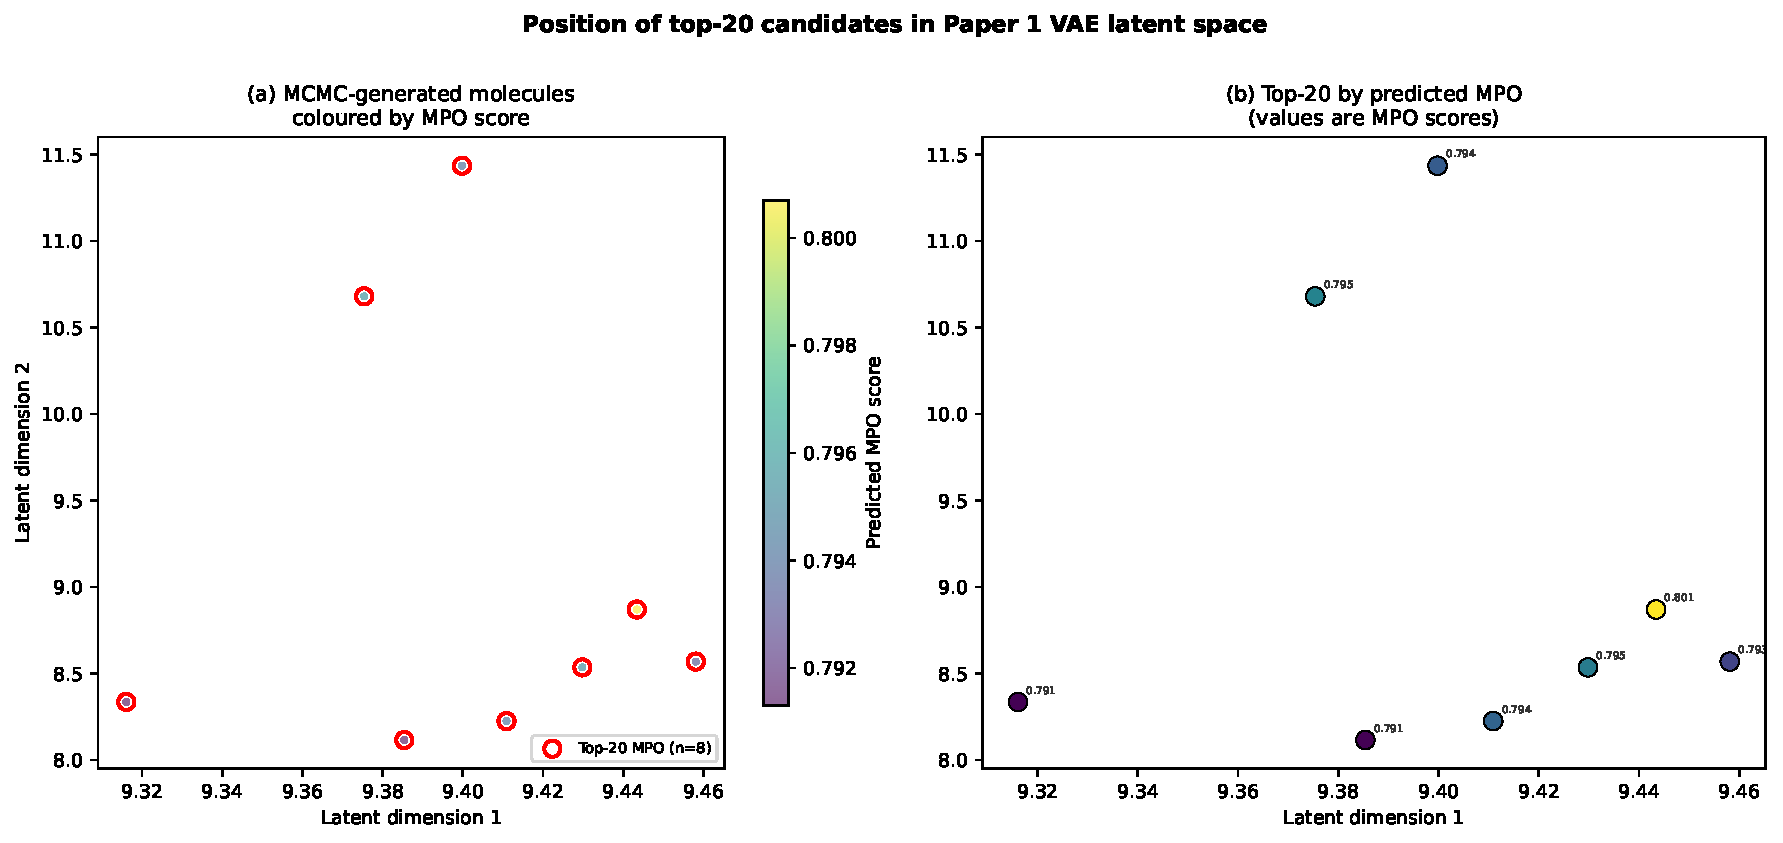
\includegraphics[width=0.75\textwidth]{VAE_latent_space.pdf}
\caption{Position of the top-20 candidates in the Paper~1 VAE latent space. Molecules are coloured by predicted MPO score; top-20 by MPO are highlighted in red.}
\label{fig:s2_vae_latent}
\end{figure}

% ============================================================================
% Table S3: MM-GBSA WT results and mutant interpretation
% ============================================================================
\begin{table}[htbp]
\centering
\caption{Endpoint-analysis interpretation for the four parent-study consensus complexes used for production MD. These systems are distinct from the 17 set-C polypharmacology candidates. Mean $\pm$ standard deviation is shown only for the single interpretable MM-GBSA result from 101 snapshots; dissociated or conversion-corrupted systems are reported as N/A. Mutant RRS is a docking-based analysis of set C and is not assigned to these MD systems.}
\label{tab:s3_mmgbsa_mutants}
\scriptsize
\begin{tabular}{l l S[table-format=-2.2] S[table-format=1.2] l}
\toprule
Ligand & Target & {$\Delta G_{\mathrm{bind}}$} & {Std. dev.} & Interpretation \\
\midrule
164 & PfClpR-labelled cohort$^\ast$-WT & {--} & {--} & N/A; ligand dissociated$^\ddagger$ \\
201 & PfDHFR-WT & {--} & {--} & N/A; ligand dissociated$^\ddagger$ \\
214 & PfCRT-WT & -18.25 & 0.40 & Interpretable (gmx\_MMPBSA) \\
438 & PfATP4-WT & {--} & {--} & N/A; conversion corrupted$^\S$ \\
\bottomrule
\multicolumn{5}{p{0.90\linewidth}}{$^\ast$PDB 4GM2 is PfClpR rather than PfClpP; the 164-labelled system is therefore not structural validation of PfClpP.} \\
\multicolumn{5}{p{0.90\linewidth}}{$^\ddagger$Ligand dissociated during production; no binding free energy is inferred.} \\
\multicolumn{5}{p{0.90\linewidth}}{$^\S$Excluded due to two-chain topology incompatibility with CHARMM36-to-AMBER conversion.} \\
\end{tabular}
\end{table}

% ============================================================================
% Table S5: Predicted ADMET profile (ADMET-AI, parent-library screening)
% ============================================================================
%% ============================================================================
%% Table S5: ADMET Cross-Validation Results
%% Target: JCIM Supplementary Information
%% Note: Data to be populated upon completion of ADMET cross-validation.
%% Columns: Compound, ADMET-AI LogS, ADMETlab 3.0 LogS, SwissADME LogS, etc.
%% ============================================================================

\begin{table}[htbp]
\centering
\caption{ADMET cross-validation for the 20 selected candidates and 5 reference controls. Predictions from three independent tools (ADMET-AI, ADMETlab 3.0, SwissADME) are compared. Spearman correlations between ADMET-AI and ADMETlab 3.0 are reported for solubility (LogS), hERG inhibition (pIC\textsubscript{50}), blood--brain barrier penetration (logBB), and CYP3A4 inhibition (probability). Compounds where any two tools disagreed by more than one risk category are flagged.}
\label{tab:s5_admet}
\begin{tabular}{l S[table-format=1.2] S[table-format=1.2] S[table-format=1.2] S[table-format=1.2] l}
\toprule
Compound & {ADMET-AI LogS} & {ADMETlab LogS} & {SwissADME LogS} & {hERG pIC\textsubscript{50}} & Flagged? \\
\midrule
\multicolumn{6}{l}{\textit{Data to be populated from three independent ADMET tools.}} \\
\bottomrule
\end{tabular}
\end{table}


% ============================================================================
% Table S6: ACSI Weight Sensitivity
% ============================================================================
%% ============================================================================
%% Table S4: ACSI Weight Sensitivity Analysis
%% ============================================================================

\begin{table}[htbp]
\centering
\caption{Candidate-cohort ACSI weight sensitivity. One ACSI component weight was varied by \qty{\pm 20}{\percent} and the remaining weights were rescaled proportionally to preserve a unit sum. Mean and standard deviation refer to the resulting ACSI values across the \num{17} candidates. Rank stability is measured by Spearman correlation over all candidates and Jaccard overlap of the top five candidates with the baseline ranking. Because the full-library component matrix was unavailable, this analysis applies only to the 17-candidate Set-C cohort; it does not assess the full-library top-20 ranking.}
\label{tab:s4_acsi_sensitivity}
\scriptsize
\begin{tabular}{l r S[table-format=1.3] S[table-format=1.3] S[table-format=1.3] S[table-format=1.4] S[table-format=1.4]}
\toprule
Weight varied & Variation (\%) & {New weight} & {Mean ACSI} & {SD} & {Spearman $\rho$} & {Top-5 Jaccard} \\
\midrule
$D_{\mathrm{DrugBank}}$ & -20 & 0.320 & 0.512 & 0.149 & 0.9779 & 0.6667 \\
$D_{\mathrm{DrugBank}}$ & +20 & 0.480 & 0.574 & 0.159 & 0.9338 & 0.6667 \\
$D_{\mathrm{ANPDB}}$    & -20 & 0.200 & 0.568 & 0.149 & 0.9167 & 0.6667 \\
$D_{\mathrm{ANPDB}}$    & +20 & 0.300 & 0.518 & 0.158 & 0.9804 & 0.6667 \\
$f_{\mathrm{sp}^3}$      & -20 & 0.160 & 0.552 & 0.152 & 0.9510 & 0.6667 \\
$f_{\mathrm{sp}^3}$      & +20 & 0.240 & 0.534 & 0.153 & 0.9583 & 0.6667 \\
$\mathrm{NPL}$            & -20 & 0.120 & 0.535 & 0.160 & 0.9632 & 0.6667 \\
$\mathrm{NPL}$            & +20 & 0.180 & 0.551 & 0.145 & 0.9804 & 1.0000 \\
\bottomrule
\end{tabular}
\end{table}


% ============================================================================
% Figure S4: RRS Radar Plots
% ============================================================================
\begin{figure}[htbp]
\centering
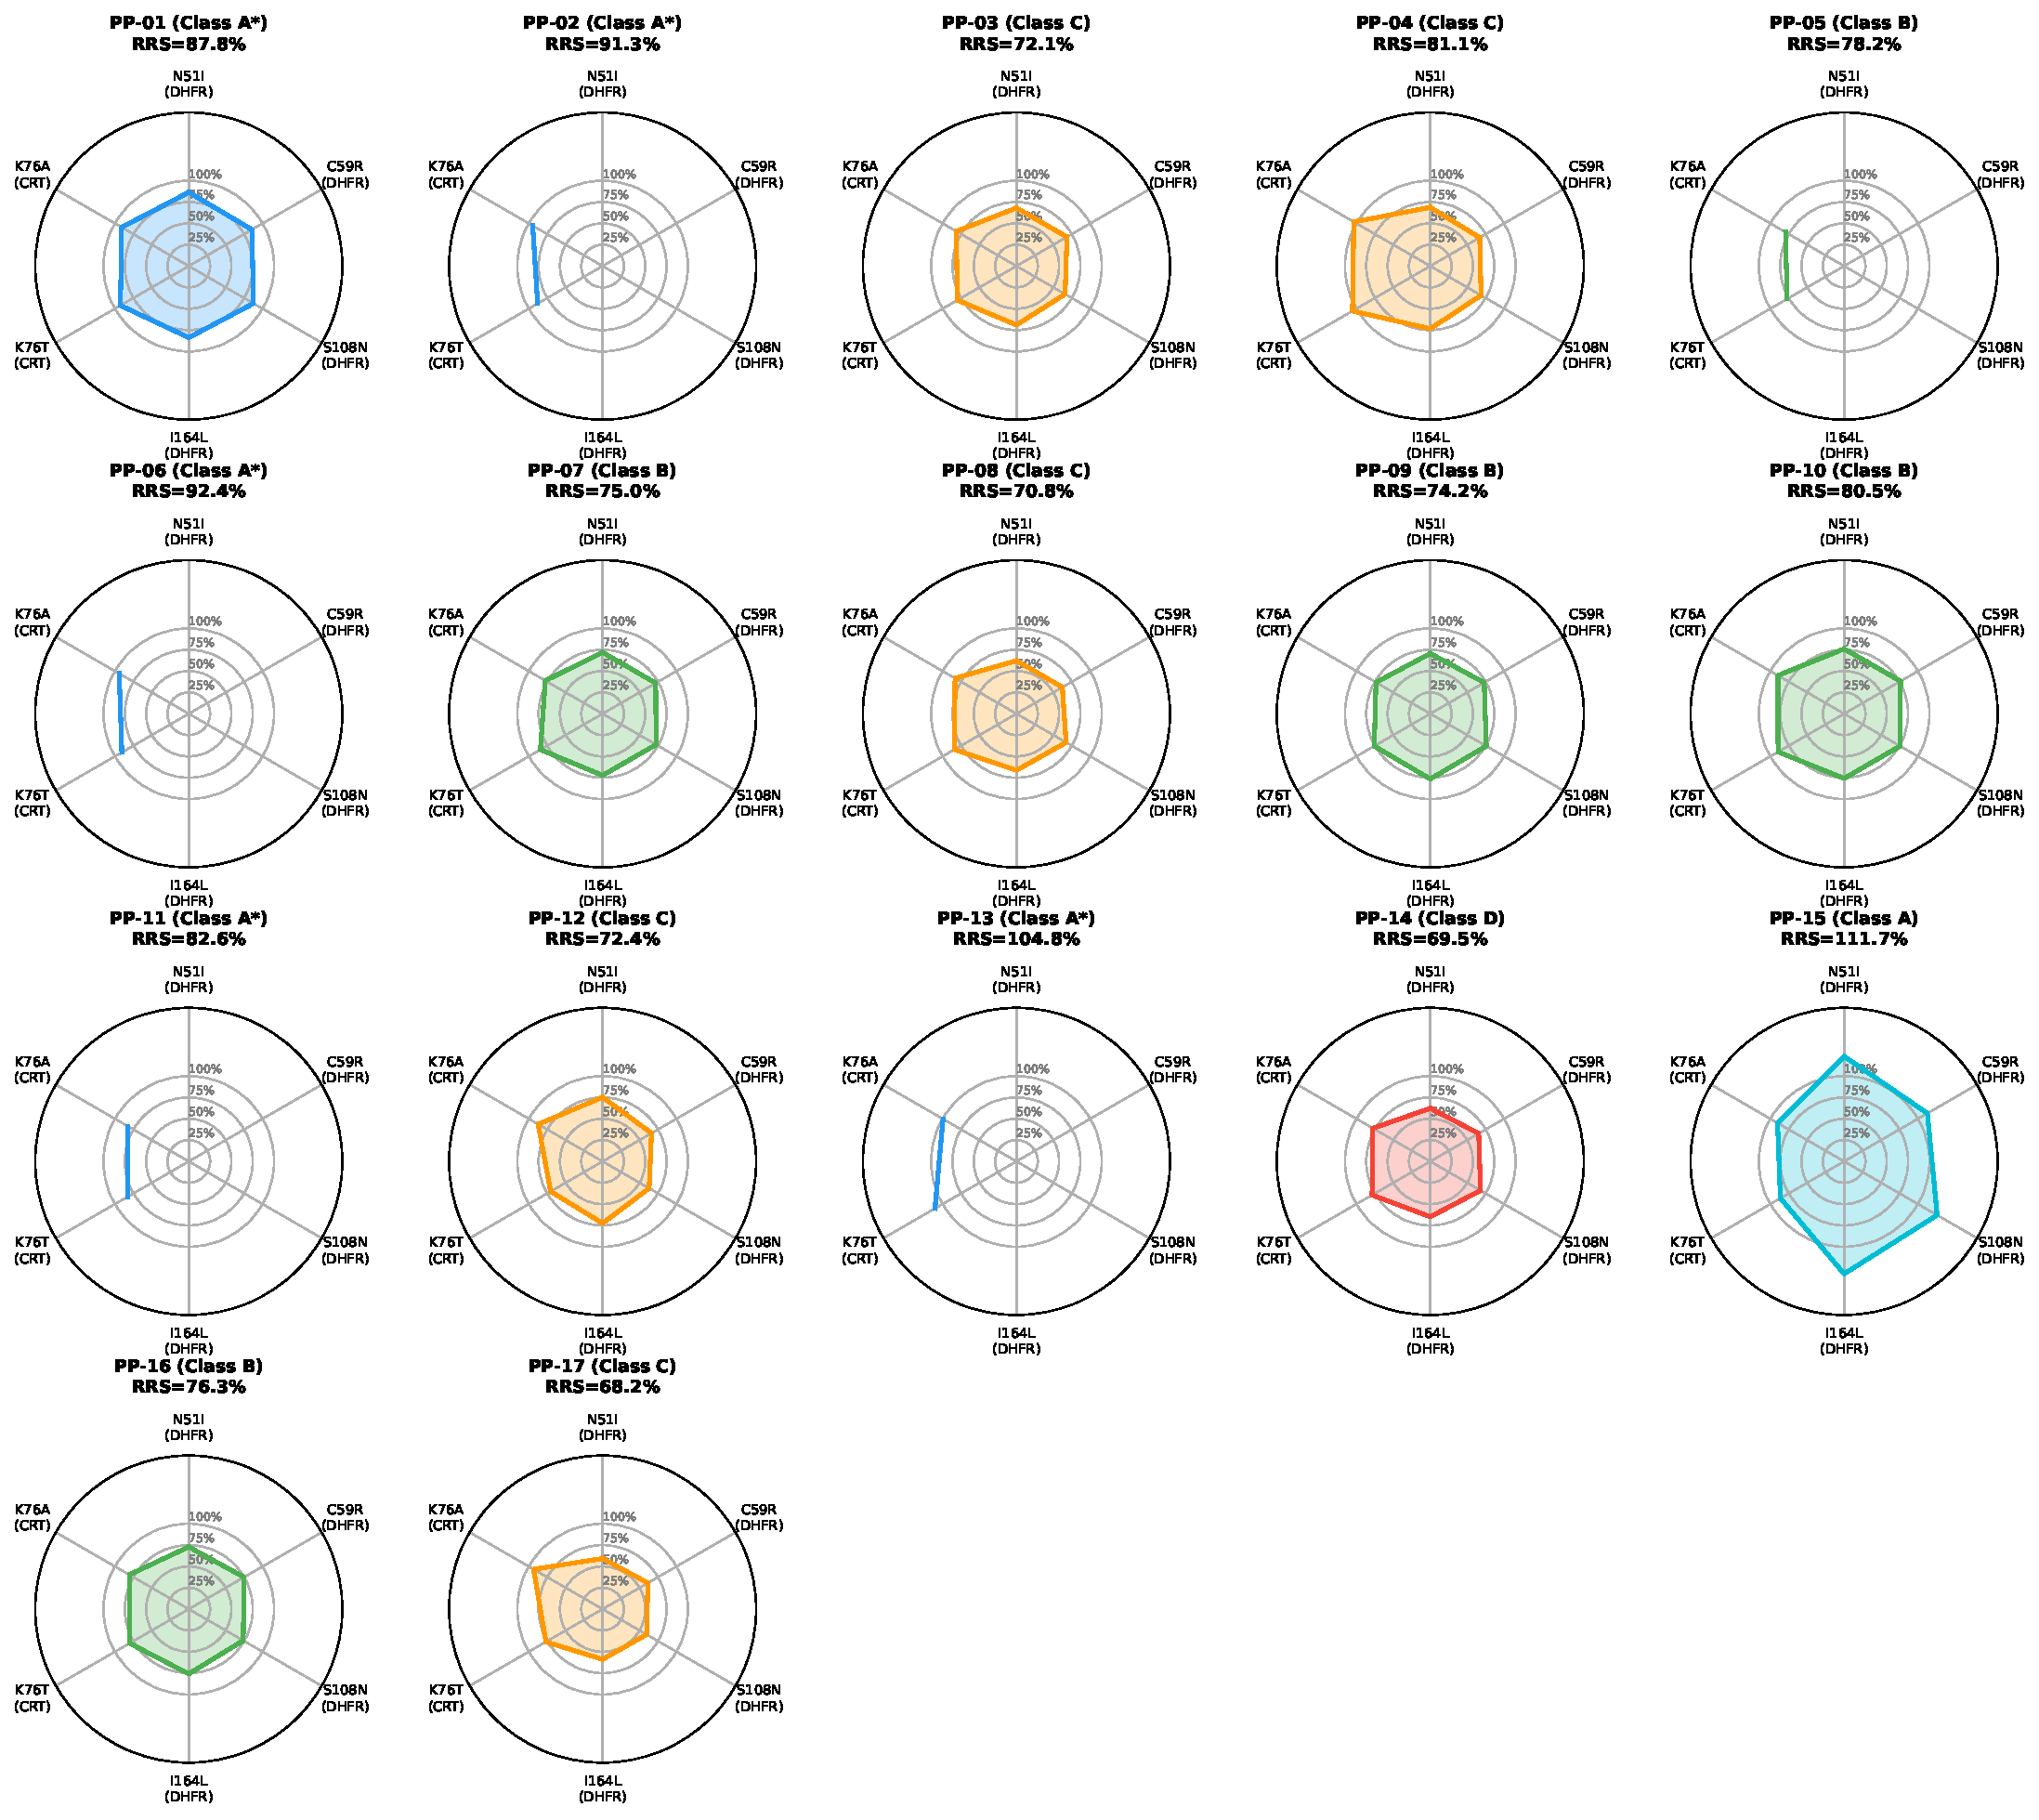
\includegraphics[width=\textwidth]{rrs_radar_profiles.pdf}
\caption{Per-compound, docking-derived RRS profiles across all six resistance mutations for the 17 set-C polypharmacological leads. The four parent-study MD systems are not included. Each axis represents one mutation; concentric rings indicate \qty{50}{\percent}, \qty{100}{\percent}, and \qty{150}{\percent} RRS (WT-normalised). Larger radial values indicate greater preservation of the docking score relative to the corresponding wild-type target; the plot does not encode absolute binding potency.}
\label{fig:s4_rrs_radar}
\end{figure}

\noindent\textit{Scope of the MD evidence.} The parent-study trajectories provide a targeted structural check on four wild-type complexes; they do not constitute candidate-specific Set-C production MD. No trajectory-derived MD-RRS estimate or mutant-state MM-GBSA result is included in this Supporting Information.

% ============================================================================
% Table S7: PlasmoDB target annotation and mutation provenance
% ============================================================================
\begin{table}[htbp]
\centering
\caption{Stable \textit{Plasmodium falciparum} target identifiers and mutation context used in this study. Identifiers are reported for annotation and provenance only; they do not constitute pathway-level target engagement, causal network evidence, or experimental validation. The accompanying source-data record preserves the target annotations and retrieval provenance.}
\label{tab:s7_plasmodb}
\begin{tabularx}{\textwidth}{l l l X}
\toprule
Target & Stable gene ID & Structural context & Mutation or evidence boundary \\
\midrule
PfDHFR & \texttt{PF3D7\_0417200} & 7F3Y WT template & N51I, C59R, S108N, I164L; antifolate-resistance states \\
PfCRT & \texttt{PF3D7\_0709000} & 6UKJ WT template & K76T clinical resistance marker; K76A comparator state \\
PfATP4 & \texttt{PF3D7\_1211900} & 9N10 parent-study structure & Target annotation only; not part of the Set-C mutation panel \\
PfClpP & \texttt{PF3D7\_0307400} & Proteolytic Clp subunit & Not assigned to PDB 4GM2; no PfClpP claim is inferred from the 4GM2 record \\
PfClpR & \texttt{PF3D7\_1436800} & 4GM2, PfClpR(P61--E244) & 4GM2 is PfClpR, not PfClpP; parent-study identity retained explicitly \\
\bottomrule
\end{tabularx}
\end{table}

The stable identifiers were retrieved from PlasmoDB/VEuPathDB annotations on 12 August 2026 \citep{plasmodb_2026}; record-level permalinks and the retrieval date are preserved in the machine-readable CSV. The exact database release/build was not captured in the source snapshot and is therefore not treated as an inferred annotation version. Because the present study does not provide an independent multi-gene targetome or a prespecified parasite-proteome background, no GO or pathway-enrichment test was performed. This table therefore supplies biological identity and mutation provenance without converting docking scores into pathway-level evidence \citep{Trapotsi2022MoA}.

% ============================================================================
% Table S8: Cohort and estimand separation
% ============================================================================
% Table S8: Cohort and estimand separation
\begin{table}[htbp]
\centering
\caption{Questions addressed and interpretation boundaries. The Set-C docking cohort has 17 candidates and 136 wild-type/mutant systems after prioritization filters; 12 candidates have complete PfDHFR/PfCRT panels and define the primary RRS analysis, and 5 are PfCRT-only records reported separately. Parent-study MD systems do not overlap Set-C. The 16-system Set-C pilot passed geometric trajectory checks and is analyzed separately; its MD-RRS and MM-GBSA values are not used to assign docking-RRS classes.}
\label{tab:s6_cohort_estimands}
\scriptsize
\begin{tabularx}{\textwidth}{>{\raggedright\arraybackslash}p{0.16\textwidth} >{\raggedright\arraybackslash}p{0.17\textwidth} >{\raggedright\arraybackslash}p{0.13\textwidth} >{\raggedright\arraybackslash}X >{\raggedright\arraybackslash}X}
\toprule
Evidence layer & Cohort & Systems & Primary analyses & Interpretation boundary \\
\midrule
Set-C docking & PP-01--PP-17 & 136 (12 complete; 5 PfCRT-only) & WT/mutant docking; target-specific RRS, ACSI, PNS & Filtered prioritisation cohort; not measured binding or MD-RRS \\
Parent-study MD & Ligands 164, 201, 214, 438 & 4 WT complexes $\times$ \SI{10}{\nano\second} & RMSD, contacts, bound-state assessment, MM-GBSA where valid & Structural check; one interpretable MM-GBSA estimate (PfCRT--214) \\
Set-C MD pilot & PP-01/PP-02 & 16 systems (all met trajectory criteria) & Trajectory geometry, MD-RRS, MM-GBSA & Single-replicate structural follow-up; separate from docking-RRS classification \\
Full Set-C MD-RRS & PP-01--PP-17 & 136 planned systems & Full trajectory QC and MD-RRS & Not available because the complete cohort was not simulated \\
\bottomrule
\end{tabularx}
\end{table}


\bibliographystyle{unsrtnat}
\bibliography{Bibliography_Polypharmacology_MD_Validation}

\section*{Use of Artificial Intelligence}

During the preparation of this work the authors used AI assistants to support code development and data analysis scripting. The authors reviewed and edited all AI-assisted output and take full responsibility for the content of this article. No generative AI tool is listed as an author. All computational results, statistical analyses, and quantitative claims were generated and verified by the authors.

\end{document}
